\documentclass[12pt]{amsart}
\usepackage{amsthm}
\usepackage{graphicx}
\usepackage[]{geometry}
\newcommand*\oct{\vcenter{\hbox{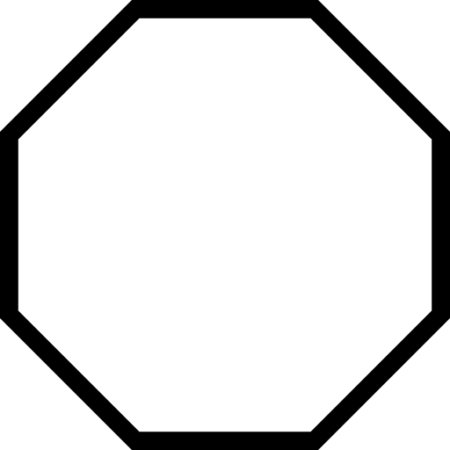
\includegraphics[width=.9em]{octagon.png}}}}
\newcommand{\F}{\mathcal{F}}
\newcommand{\Z}{\mathbb{Z}}
\usepackage[]{hyperref}

\newtheorem{theorem}{Theorem}
\newtheorem{lemma}{Lemma}
\newtheorem{proposition}{Proposition}
\newtheorem{corollary}{Corollary}

\theoremstyle{definition}
\newtheorem{definition}{Definition}

\title{Stopped Binary Strings}
\author{Robert Dougherty-Bliss and Charles Kenney}

\begin{document}
\maketitle

\begin{abstract}
    A binary string $(x_1, \dots, x_n)$ is \emph{stopped at index $k$} if all
    indices in $(k / 2, k]$ are zero. The \emph{stopping time} of a binary
    string is the smallest such $k$, if any exist. We show that the number of
    binary strings of length $2n$ with stopping time $2n$ is the $n$th
    Narayana--Zidek--Cappel number. By considering binary expansions, we
    produce two new integer sequences (the ``stopped'' integers) and a
    measurable subset of the unit interval with unknown measure. Generalizing
    these results to arbitrary bases produces infinite families of integer
    sequences not in the OEIS and infinitely many new constants denoting the
    measures of certain sets of the unit interval.
\end{abstract}

\noindent A new, experimental machine is placed into a factory. Despite its
inventor's extolments, management is skeptical. They subject the machine to a
rigorous \emph{testing} process: Once a week, an inspector will visit the
machine and mark down a $1$ if a problem is detected, and a $0$ otherwise. The
first time the machine passes exactly half of its total inspections,
inspections will cease. This process creates a \emph{binary string}, and the
question at hand is whether it ends in sufficiently many $0$'s to denote a
successful testing regimen. We call such successful binary string
\emph{stopped}. Some questions are immediate: Given a fixed number of
inspections, how many binary strings are stopped? If we inspect \emph{forever},
how many inspections will eventually result in a stopped string? And so on.
This paper explores some of these questions. Along the way we will produce an
infinite family of sequences which do not appear in the OEIS, an infinite
family of measurable sets on the real line whose measures are unknown, and two
particular integer sequences which do not appear in the OEIS.

A binary string $(x_1, x_2, \dots x_n)$ is said to be \emph{stopped at index $k
\leq n$} if $x_j = 0$ for all $j \in (k / 2, k]$. The \emph{stopping time} of a
binary string is the smallest $k$ such that the string is stopped at index $k$,
or $\infty$ if no such $k$ exists. Note that, except $1$ and $\infty$, every
stopping time is even. We call a string of length $n$ with stopping time $n$
``stopped'' without reference to an index. 

The motivating result for this paper is that the number of binary sequences of
length $2n$ with stopping time $2n$ equals the $n$th Narayana--Zidek--Cappel
number $T_n$, defined by the recurrence
\begin{align*}
    T_1 &= 1 \\
    T_2 &= 1 \\
    T_{2n} &= 2 T_{2n - 1} \\
    T_{2n + 1} &= 2 T_{2n} - T_n.
\end{align*}
This sequence is A2083 in the OEIS \cite{oeis}. It originates from
\cite{capell1970knock}, where the authors show that $T_n$ enumerates the number
of random knock-out tournaments with $n$ players.

Alongside this result, our definition of a stopped string generalizes to
various integer sequences and sets of reals by passing to the relevant binary
expansions. The definition also generalizes to bases other than $2$, the only
change being that any occurrence of ``$1$'' should be replaced with ``any
nonzero digit.'' This leads to an infinite family of sets, integer sequences,
and so on.

The rest of this paper is organized as follows. Section~\ref{sec:recs}
establishes the identity between the number of stopped binary strings and the
Narayana--Zidek--Capell numbers, generalizes this result to arbitrary bases,
and gives some elementary results about the enumerating sequences.
Section~\ref{sec:reals} defines a set of reals in the unit interval whose
binary expansions are ``stopped,'' and considers the measure of this set.
Section~\ref{sec:integers} gives two new integer sequences and discusses their
natural densities.

\section{Counting stopped binary strings}%
\label{sec:recs}

Let $g(n)$ be the number of binary strings of length $n$ with stopping time
$n$. Since stopping times are even except for $1$, we know that $g(n)$ is zero
for all odd $n$ except $n = 1$, where $g(1) = 1$. Thus the interesting sequence
is $a(n) = g(2n)$, which we will show (in two ways!) equals the
Narayana--Zidek--Capell numbers.

It is convenient to work with \emph{infinite} binary strings which are nonzero
in only finitely many places. This is equivalent to studying finite binary
strings, but has the benefit that every such infinite string has a finite
stopping time when considered as a sufficiently long, finite binary string.

\begin{definition}
    Let
    \begin{equation*}
        V = \bigoplus_{k=1}^\infty (\Z/2\Z)
    \end{equation*}
    be the direct sum of infinitely many copies of $\Z / 2\Z$. That is, the set
    of all infinite tuples $(x_1, x_2, x_3, \dots)$ where each $x_k$ is $0$ or
    $1$, and only finitely many are $1$. For each positive integer $k$, let
    $\oct_k$ be the set of elements of $V$ which are zero beyond position $k$
    and, when the first $k$ entries are regarded as a finite binary string,
    they have stopping time $k$. That is, $\oct_1 = \{0\} \subset V$,
    \begin{equation*}
        \oct_{2k} = \{v \in V : \forall j > k, v_j = 0, \text{ and } v \text{ has stopping time } 2k \}
    \end{equation*}
    and $\oct_{2k + 1} = \emptyset$ for every integer $k \geq 1$.
\end{definition}

Note that $g(n) = |\oct_n|$ for every positive integer $n$.

\begin{theorem}
    The sequence $g(n)$ satisfies the recurrence
    \begin{align*}
        g(1) &= g(2) = g(4) = 1 \\
        g(4n) &= 2 g(4n - 2) \\
        g(4n + 2) &= 2 g(4n) - g(2n).
    \end{align*}
\end{theorem}

First, we will prove this directly from our definitions.

\begin{proof}
    Each nonzero element in $V$ has a final nonzero entry (a $1$). Let $e_0
    \colon V \to V$ be a map which inserts a $0$ in the position of this final
    entry, shifting the previous final entry to the right one space. Similarly,
    let $e_1$ insert a $1$. Symbolically,
    \begin{equation*}
        e_0(b) =
            \begin{cases}
                0 \text{ if } b=0 \\
                (b_1, ..., b_j, 0, 1, 0,0,...) \text{ if } b = (b_1, ..., b_j, 1, 0, 0, ...)
            \end{cases}
    \end{equation*}
    and
    \begin{equation*}
        e_1(b) =
            \begin{cases}
                (1, 0, 0, \dots) \text{ if } b=0 \\
                (b_1, ..., b_j, 1, 1, 0,0,...) \text{ if } b = (b_1, ..., b_j, 1, 0, 0, ...).
            \end{cases}
    \end{equation*}
    Note that $e_0$ and $e_1$ are injective, $e_0(V) \cap e_1(V) = \emptyset,$
    and $e_0(V) \cup e_1(V) = V.$

    For any positive integer $k$,
    \begin{equation*}
        \oct_{2k + 2} \subseteq e_0(\oct_{2k}) \cup e_1(\oct_{2k}).
    \end{equation*}
    Indeed, the final nonzero entry of every string in $\oct_{2k + 2}$ occurs
    at position $k + 1$. Removing the immediately preceding entry produces a
    string in $\oct_{2k}$---$e_0$ and $e_1$ simply add the entry back.

    In the other direction, for $k \geq 2$ we have
    \begin{equation*}
        e_1(\oct_{2k}) \subseteq \oct_{2k + 2},
    \end{equation*}
    because inserting a $1$ into position $k$ will never decrease the stopping
    time. For \emph{odd} $k \geq 3$ we have
    \begin{equation*}
        e_0(\oct_{2k}) \subseteq \oct_{2k + 2},
    \end{equation*}
    because inserting a $0$ at position $k$ will only decrease the stopping
    time if the new stopping time \emph{is} $k$; this is impossible if $k$ is
    odd. This shows that
    \begin{equation*}
        \oct_{2k + 2} = e_0(\oct_{2k}) \cup e_1(\oct_{2k}),
    \end{equation*}
    and thus
    \begin{equation*}
        g(2k + 2) = 2 g(2k)
    \end{equation*}
    for $k$ odd.

    To handle the even case, let
    \begin{equation*}
        \oct_{2k}^1 = \{(b_1, ..., b_{2k}, 1, 0,0,...) \in V \text{ s.t. } (b_1,...,b_{2k},0,0,...) \in \oct_{2k}\}.
    \end{equation*}
    (Note that $|\oct_{2k}^1| = |\oct_{2k}| = g(2k)$.) Then
    \begin{equation*}
        e_0(\oct_{4k}) \subseteq \oct_{4k + 2} \cup \oct_{2k}^1.
    \end{equation*}
    This implies
    \begin{equation*}
        \oct_{4k + 2} \cup \oct_{2k}^1 = e_0(\oct_{4k}) \cup e_1(\oct_{4k}).
    \end{equation*}
    (That the left contains the right is clear given the preceding inclusion.
    For the other direction, note $\oct_{2k}^1 \subseteq
    e_0(\oct_{4k})$, since if $(b_1, ..., b_{2k}, 0,0,...) \in \oct_{2k}$ then
    $(b_1, ..., b_{2k-1},1,0,0,...)$ has stopping time precisely $4k$.) Therefore
    \begin{equation*}
        g(4k + 2) + |\oct_{2k}^1| = 2 g(4k),
    \end{equation*}
    or
    \begin{equation*}
        g(4k + 2) = 2 g(4k) - g(2k).
    \end{equation*}
    This establishes the recurrence.
\end{proof}

Now we will prove our theorem combinatorially by relating our sequence to a
certain class of compositions. Recall that a \emph{composition} of an integer
$n$ is a vector in $(\Z_{>0})^m$, for some $m \in \{1,2,...,n\},$ whose
components add to $n$. The $n$th Narayana-Zidek-Capell number, $a(n)$, is the
cardinality of the set
\begin{align*}
    R_n = \left\{ \text{Compositions } p \text{ of } n \text{ satisfying } p_1 = 1 \text{ and } p_k \leq \sum_{j=1}^{k-1} p_j \right\}.
\end{align*}
%OEIS reference for this, or better yet the original source

\begin{proof}
    For $j \in \Z_{>0},$ let $f(j) = (0,0,...,0,1)$, with $j-1$ zeroes preceding the one.
    Then for $p \in (\Z_{>0})^m,$ let
    \begin{align*}
        F(p) = (f(p_1), f(p_2), ..., f(p_m), 0,0,...),
    \end{align*}
    concatenated in the natural way, with a tail of zeroes appended at the end.
    Then $F: R_n \overset{\sim}{\to} \oct_{2n}$ is a bijection, so $|\oct_{2n}| = g(2n) = a(n).$
    Indeed, if $p \in R_n$, then since $\sum_{j=1}^{m} p_j = n,$ the final nonzero entry in $F(p)$ is in spot $n$. Thus
    $F(p)$ is stopped at time $2n$, and is not stopped at time $t$ for any $t \in [n,2n-1].$
    And if the zeroes from $f(p_r)$ in $F(p)$ caused $F(p)$ to be stopped at some time $t \leq n-1,$
    \begin{align*}
        F(p) = (f(p_1), ..., f(p_{r-1}), 0,0,...,&0,...) \\
	&\uparrow \\
	&\text{index } t
    \end{align*}
    then $p_r  > \lceil t/2 \rceil \geq \sum_{j=1}^{r-1} p_j.$ But this would contradict the fact that $p \in R_n.$
    And, if $b \in \oct_{2n}$ has 1s at indices $a_1 = 1, a_2, ..., a_\ell = n,$ then
    \begin{align*}
	&F^{-1}: \oct_{2n} \to R_n \\
	&F^{-1} : b \mapsto (a_1, a_2 - a_1, a_3 - a_2, ..., a_\ell - a_{\ell-1})
    \end{align*}
    provides an inverse to $F$, since the index $a_r$ of the $r$th one in b is at most
    twice the index $a_{r-1}$ of the $(r-1)$st one.
\end{proof}

A slightly different recurrence holds for arbitrary bases. Let $g_b(n)$ be the
number of $b$-ary strings of length $n$ with stopping time $n$. Then
\begin{align*}
    g_b(1) &= 1 \\
    g_b(2) &= b - 1 \\
    g_b(4) &= (b - 1)^2 \\
    g_b(4n) &= b g_b(4n - 2) \\
    g_b(4n + 2) &= b g_b(4n) - (b - 1) g_b(2n).
\end{align*}

For convenience, let $r_b(n) = g_b(2n)$, so that the recurrences read
\begin{align*}
    r_b(1) &= b - 1 \\
    r_b(2) &= (b - 1)^2 \\
    r_b(2n) &= b r_b(2n - 1) \\
    r_b(2n + 1) &= b r_b(2n) - (b - 1) r_b(n).
\end{align*}

The sequences $r_b(n)$ seem new for $b \geq 3$ in the sense that they do not
appear in the OEIS. All $r_b(n)$ satisfy the following ``meta-Fibonacci''
property.

\begin{proposition}
    For all $b \geq 2$ and $n \geq 2$,
    \begin{equation*}
        r_b(n) = (b - 1) \sum_{k = 1}^{\lfloor n / 2 \rfloor} r_b(n - k).
    \end{equation*}
\end{proposition}

\begin{proof}
    The result holds for $n = 2$ since
    \begin{equation*}
        r_b(2) = (b - 1) \sum_{k = 1}^1 r_b(k).
    \end{equation*}
    For $2n \geq 4$, we can use induction to write
    \begin{align*}
        r_b(2n) &= (b - 1) r_b(2n - 1) + r_b(2n - 1) \\
                &= (b - 1) r_b(2n - 1) + (b - 1) \sum_{k = 1}^{n - 1} r_b(2n - 1 - k) \\
                &= (b - 1) \sum_{k = 1}^n r_b(2n - k).
    \end{align*}
    A similar argument applies for $2n + 1 \geq 3$.
\end{proof}

Meta-Fibonacci sequences are those whose terms are generated by summing some
number of the previous terms. Specifically, a sequence $a(n)$ is
$p(n)$-Fibonacci if
\begin{equation*}
    a(n) = \sum_{k = 1}^{p(n)} a(n - k).
\end{equation*}
Our previous proposition shows that $r_2(n)$, the Narayana--Zidek--Capell
numbers, is a meta-Fibonacci sequence. This fact is well-known and can be used
to show that $r_2(n) / 2^n$ converges to a positive constant (see
\cite{emerson2006family}). However, sequences of the form
\begin{equation*}
    a(n) = \alpha \sum_{k = 1}^{p(n)} a(n - k)
\end{equation*}
seem to be unstudied for $\alpha \neq 1$.

\begin{proposition}
    For every $b \geq 2$, $g_b(2n) / b^n$ is monotonically decreasing. In
    particular,
    \begin{equation*}
        \frac{g_b(2n)}{b^n} \leq \frac{b - 1}{b}
    \end{equation*}
    for $n \geq 1$.
\end{proposition}

\begin{proof}
    Since $g_b(2n)$ is positive by definition, the recurrence for $g_b(2n)$
    implies
    \begin{equation*}
        g_b(2n) \leq b g_b(2n - 2)
    \end{equation*}
    for all $n \geq 2$, which is equivalent to our claim that $g_b(2n) / b^n$
    is monotonically decreasing. In particular,
    \begin{equation*}
        \frac{g_b(2n)}{b^n} \leq \frac{g_b(2)}{b^1} = \frac{b - 1}{b},
    \end{equation*}
    as desired.
\end{proof}

Our proposition implies that $g_b(2n) / b^n$ converges to some nonnegative
constant, and we suspect that it is a \emph{positive} constant. As we have
said, the case $b = 2$ generates the Narayana--Zidek--Capell numbers $a(n)$,
and it is well-known that $a(n) / 2^n$ converges to a positive constant. See,
for example, Capel and Narayana original paper \cite{capell1970knock}, or
Emerson's argument in \cite{emerson2006family}. (According to the OEIS, the
constant is exactly twice the Atkinson-Negro-Santoro constant given in Section
2.28 of Finch's book of mathematical constants \cite{finch2003mathematical}.)

\section{Stopped reals in the unit interval}
\label{sec:reals}

Every element of the unit interval $[0, 1]$ can be regarded, via its binary
expansion, as an infinite binary string, i.e., an element of $\Z / 2 Z \times
\Z / 2Z \times \cdots$. This differs from the set $V$ of the previous section
by allowing potentially infinitely many nonzero entries. For example, the real
\begin{equation*}
    (0.1010101010101\dots)_2 = \frac{2}{3}
\end{equation*}
is perfectly well-defined, but not as a member of $\bigoplus_{k = 1}^\infty (\Z
/ 2 \Z)$. In this way, it makes since to discuss stopped \emph{reals},
considering each real as an infinite binary string. (We shall interchangably
refer to reals as both strings and numbers.) Our focus now becomes
\emph{topological} as we examine the \emph{set} of stopped reals in the unit
interval.

\begin{definition}
    Let $S_k$ be the set of reals in $[0, 1]$ which have stopping time $k$ when
    regarded as an infinite binary string. Membership in this set is determined
    by examining only the first $k$ bits of a binary expansion, so $S_k$ is
    measureable. Let $S = \cup_{k \geq 1} S_k$ be the set of all stopped reals
    in $[0, 1]$, which is measurable since the $S_k$ are.
\end{definition}

Let us get a feel for what the sets $S_k$ ``look like.'' First, observe that
every element of $S_k$ consists of a binary string which has stopping time $k$
followed by \emph{any} binary string at all. Thus, each string with stopping
time $k$ determines an interval of length $2^{-k}$ included in $S_k$, and the
disjoint union of these intervals is \emph{all} of $S_k$. In this way, we can
compute the following sets:
\begin{align*}
    S_1 &= [0, 1/2) \\
    S_2 &= [1/2, 3/4) \\
    S_4 &= [3/4, 13/16) \\
    S_6 &= [7/8, 57/64) \\
    S_8 = [13/16, 209/256) &\cup [15/16, 241/256).
\end{align*}

[Insert the stopping time plot somewhere around here.]

This simple description of $S_k$ gives us a nice expression for the measure of
$S$.

\begin{theorem}
    Let $\beta_2$ be the measure of $S$. Then
    \begin{equation*}
        \beta_2 = \sum_{k \geq 1} \frac{g(k)}{2^k} = \frac{1}{2} + \sum_{k \geq 1} \frac{g(2k)}{4^k}
        \approx 0.841657913173647.
    \end{equation*}
\end{theorem}

\begin{proof}
    The measure of $S_k$ is $g(k) / 2^{2k}$, where $g(k)$ is the number of
    binary strings of length $k$ with stopping time $k$. Since $S$ is the
    pairwise disjoint union of the $S_k$, the ``exact'' result follows
    immediately.
\end{proof}

In the previous section we established that the sequence $a(n) = g(2n)$ is
A2083 in the OEIS. It is known that $a(n) = O(2^n)$, so the above series
converges very quickly. Using the recurrence of the previous section to
generate the first hundred terms of $g(2k)$ it is easy to approximate the sum
and provide rigorous lower bounds. To get more rigorous upper bounds, first
note $g(2n) / 2^n$ is monotonically decreasing. This implies that the error of
using
\begin{equation*}
    \frac{1}{2} + \sum_{1 \leq k < n} \frac{g(2k)}{4^k}
\end{equation*}
as an approximation to the measure of $S$ is
\begin{equation*}
    \sum_{k \geq n} \frac{g(2k)}{4^k}
        \leq \frac{g(2n)}{2^n} \sum_{k \geq n} \frac{1}{2^k}
        = \frac{2g(2n)}{4^n}
        = O(1/2^n).
\end{equation*}
For example, using the first $99$ terms ($n = 100$) will give an error of no
more than
\begin{equation*}
    \frac{22284668265087}{158456325028528675187087900672}
    \approx 1.406360286 \times 10^{-16}.
\end{equation*}

The constant $\beta_2$ seems new. Accordingly, we conjecture that it is
irrational and even transcendental, but we really know nothing about it. The
only information we have is that it is a value of the ordinary generating
function of $g(n)$.

\begin{definition}
    Let
    \begin{equation*}
        G(z) = \sum_{k \geq 0} g(k) z^k = z + \sum_{k \geq 1} g(2k) z^{2k}
    \end{equation*}
    be the ordinary generating function of $g(n)$, and
    \begin{equation*}
        A(z) = \sum_{k \geq 1} g(2k) z^k
    \end{equation*}
    the ordinary generating function of $g(2k)$. Note that $G(z) = z + A(z^2)$.
\end{definition}

\begin{proposition}
    The generating function $A(z)$ is analytic on a disk of radius $1 / 2$
    centered at the origin and satisfies
    \begin{equation*}
        A(z) = \frac{z(1 - A(z^2))}{1 - 2z}.
    \end{equation*}
\end{proposition}

\begin{proof}
    The equation is a routine computation using the recurrence for $g(2n)$ proved in
    the previous section. For convenience, let $a(n) = g(2n)$. Then:
    \begin{align*}
        \sum_{k \geq 1} a(k) z^k
            &= \sum_{k \geq 1} a(2k) z^{2k} + \sum_{k \geq 0} a(2k + 1) z^{2k + 1} \\
            &= \sum_{k \geq 1} 2 a(2k - 1) z^{2k} + a(1) z + \sum_{k \geq 1} (2a(2k) - a(k)) z^{2k + 1} \\
            &= 2 z \sum_{k \geq 0} a(2k + 1) z^{2k + 1} + 2 z \sum_{k \geq 1} a(2k) z^{2k} - z A(z^2) + z \\
            &= 2z A(z) + z(1 - A(z^2)).
    \end{align*}
    Solving this for $A(z)$ yields the result. Since $a(n) =
    O(2^n)$, we see that $A(z)$ converges everywhere that $\sum_{k \geq 0} (2z)^k = (1 -
    2z)^{-1}$ does, which is at least a disk of radius $1/2$.
\end{proof}

It is clear that
\begin{equation*}
    \beta_2 = G(1/2) =\frac{1}{2} + A(1/4).
\end{equation*}
But again, this is very little information. We suspect that neither $A(z)$ nor
$G(z)$ are algebraic.

Expanding reals in $[0, 1]$ with different bases yields different ``stopped
sets'' and different measures. The same arguments apply, except now the measure
of the $S_k$ will be $g_b(k) / b^k$. Thus, the measure of the set of $b$-ary
stopped reals is
\begin{equation*}
    \beta_b = \frac{1}{b} + \sum_{k \geq 1} \frac{g_b(2k)}{b^{2k}}.
\end{equation*}
These constants go as follows:
\begin{align*}
    \beta_2 &= 0.84165791317364708989 \\
    \beta_3 &= 0.62119074589923243760 \\
    \beta_4 &= 0.48141057151328202149 \\
    \beta_5 &= 0.39071175514852239829 \\
    \beta_6 &= 0.32805820924751380527.
\end{align*}
These seem to be decreasing, and indeed they are, down to 0.

% TODO
% Conjecture: \beta_b = 2 / b + O(1/b^n) for all n.
\begin{theorem}
    For $b \geq 2$,
    \begin{equation*}
        \frac{2}{b} - \frac{1}{b^2} \leq \beta_b \leq \frac{2}{b}.
    \end{equation*}
\end{theorem}

\begin{proof}
    The definition of $g_b$ shows that it is positive, and the recurrence
    established in the previous section shows that $g_b(2k) / b^k$ is
    monotonically decreasing. In particular,
    \begin{equation*}
        g_b(2k) / b^k \leq g_b(2) / b = \frac{b - 1}{b}.
    \end{equation*}
    for $k \geq 1$. Therefore
    \begin{equation*}
        \beta_b \leq \frac{1}{b} + \frac{b - 1}{b} \sum_{k \geq 1} \frac{1}{b^k}
        = \frac{2}{b}.
    \end{equation*}
    The lower bound is from the definition of $\beta_b$.
\end{proof}

\section{Stopped integers}
\label{sec:integers}

In this section we define two integer sequences related to stopped binary
strings. They are the \emph{maximally stopped} and \emph{prestopped} integers.

\begin{definition}
    A positive integer $n$ is \emph{maximally stopped} provided that its binary
    expansion has stopping time equal to its length. A positive integer $n$ is
    \emph{prestopped} if its binary expansion has length $k$ and is the prefix
    of a binary string with stopping time $2k$.
\end{definition}

The maximally stopped integers begin
\begin{equation*}
    2, 12, 56, 208, 240, 864, 928, 992, 3392, 3520, 3648, \dots,
\end{equation*}
and the prestopped integers begin
\begin{equation*}
    2, 4, 5, 8, 9, 10, 11, 12, 16, 17, 18, 19, 20, 21, 22, 23, 24, 25, 32, 33, \dots
\end{equation*}
Neither sequence appears in the OEIS.

\begin{definition}
    Let $M(x)$ and $P(x)$ be the number of maximally stopped and prestopped
    integers $\leq x$, respectively.
\end{definition}

\begin{proposition}
    The counting functions $M(x)$ and $P(x)$ satisfy
    \begin{equation*}
        P(x) = \Theta(M(x^2)),
    \end{equation*}
    i.e., $cM(x^2) \leq P(x) \leq C M(x^2)$ for some constants $c$ and $C$.
\end{proposition}

\begin{proof}
\end{proof}

\begin{proposition}
    The counting functions $M(x)$ and $P(x)$ satisfy
    \begin{align*}
        M(x) &= \Theta(\sqrt{x}) \\
        P(x) &= \Theta(x).
    \end{align*}
\end{proposition}

\begin{proof}
    Since $M(x) = M(\lfloor x \rfloor)$, suppose that $x$ is an integer and
    write $x = 2^m + k$ for an integer $m \geq 0$ and $0 \leq k < 2^m$. Every
    maximally stopped integer not exceeding $x$ has a binary expansion with
    length not exceeding $m + 1$. Conversely, every such binary string
    corresponds to a unique maximally stopped integer. Every such string with
    length less than $m + 1$ corresponds to an integer $< x$, so
    \begin{equation*}
        M(x) \geq \sum_{k < m + 1} g(k).
    \end{equation*}
    On the other hand, every integer counted by $M(x)$ has length $\leq m + 1$,
    so
    \begin{equation*}
        M(x) \leq \sum_{k \leq m + 1} g(k).
    \end{equation*}
    Since $g(2k) = \Theta(2^k)$, the upper bound and lower bounds are both
    $\Theta(2^{m / 2}) = \Theta(\sqrt{x})$. For example,
    \begin{equation*}
        \sum_{k \leq m + 1} g(k) = \Theta(1) + \Theta(\sum_{k \leq (m + 1) / 2} 2^k) = \Theta(2^{m / 2}) = \Theta(\sqrt{x}).
    \end{equation*}
    It follows that $M(x) = \Theta(\sqrt{x})$. This implies $M(x) / x =
    O(x^{-1/2})$, so $M(x) / x \to 0$ as $x \to \infty$.
\end{proof}

An easy corollary of this result is that the maximally stopped integers grow
like squares. That is, the $n$th maximally stopped integer is $\Theta(n^2)$. To
establish, say, the lower bound, let $m$ be the $n$th maximally stopped
integer, and note that
\begin{equation*}
    n = M(m) \leq c \sqrt{m}
\end{equation*}
for some constant $c$. Then $m \geq n^2 / c^2$. The upper bound is the same
except for the constant.

\begin{corollary}
    The maximally stopped integers have natural density $0$, i.e., $\lim_{x \to
    \infty} M(x) / x = 0$. The prestopped integers do not have natural density
    $0$.
\end{corollary}

\begin{proof}
    Since $M(x) = \Theta(\sqrt{x})$, we have $M(x) / x = \Theta(x^{-1/2})$, so
    $M(x) / x \to 0$ as $x \to \infty$. On the other hand, $P(x) = \Theta(x)$
    implies that
    \begin{equation*}
        cx \leq P(x) \leq Cx
    \end{equation*}
    for some positive constants $c$ and $C$. Thus $P(x) / x$ does \emph{not} go
    to $0$ as $x \to \infty$.
\end{proof}

\section{Conclusions and open questions}%
\label{sec:conclusion}

We have produced an infinite family of integer sequences, $g_b(n)$, an infinite
family of real constants, $\beta_b$, and two new integer sequences, the
maximally stopped and prestopped integers. These objects have left some open
questions.

We can very quickly approximate the measures $\beta_b$ using their series
representation, but we do not know much about them. Are they expressible in
terms of well-known constants such as $e$, $\pi$, and $\gamma$? Are they
irrational or transcendental?

The prestopped integers introduced in Section~\ref{sec:integers} do not have
natural density zero. Do they have \emph{any} natural density? If not, what are
their upper and lower natural densities?

\bibliographystyle{unsrt}
\bibliography{cite}

\end{document}
